\documentclass[border=6pt]{standalone}
\usepackage{tikz}
\usetikzlibrary{arrows.meta,calc,positioning}
\begin{document}
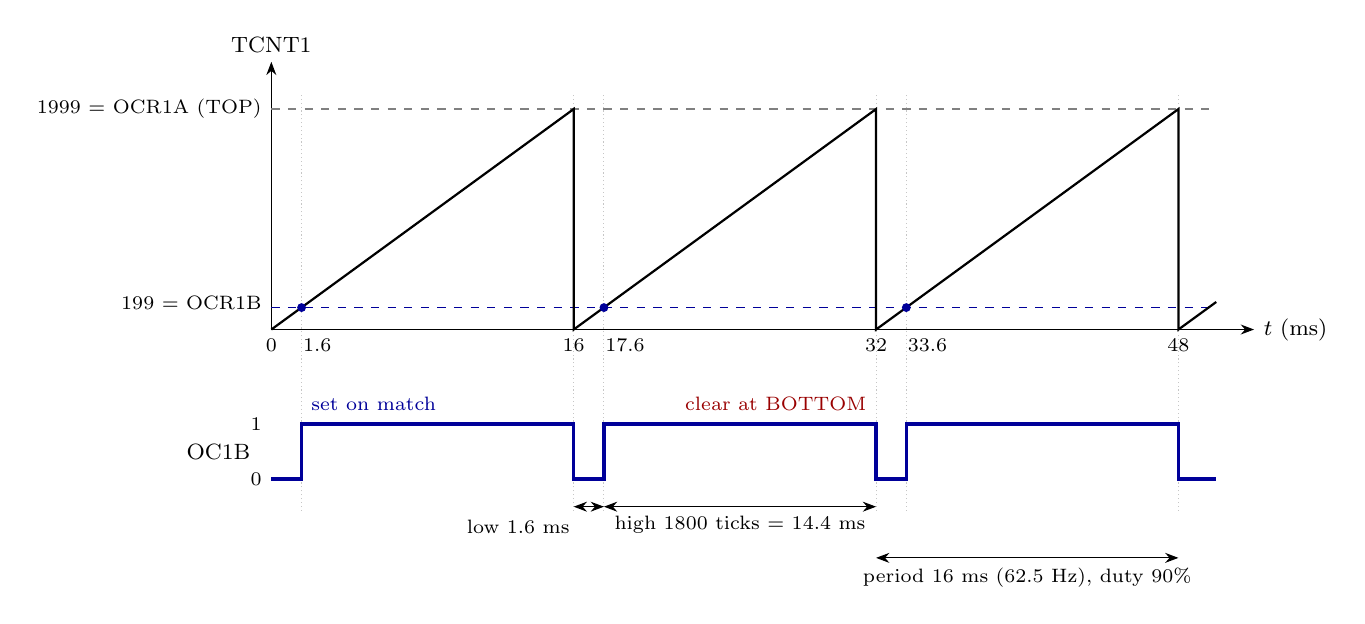
\begin{tikzpicture}[>=Stealth,font=\small,x=0.24cm,y=1cm]
% 1 unit = 1 ms; tick = 8 us; period = 2000 ticks = 16 ms; OCR1B = 199 match after 200 ticks = 1.6 ms
\def\H{2.8}\def\C{0.2787}% 199 -> 2.8*199/1999
\foreach \t in {1.6,16,17.6,32,33.6,48} \draw[gray!45,densely dotted] (\t,-2.3) -- (\t,\H+0.2);
\draw[->] (0,0) -- (0,\H+0.6) node[above,font=\footnotesize]{TCNT1};
\draw[->] (0,0) -- (52,0) node[right,font=\footnotesize]{$t$ (ms)};
\node[anchor=east,font=\scriptsize] at (0,\H) {1999 = OCR1A (TOP)};
\node[anchor=east,font=\scriptsize] at (0,\C+0.06) {199 = OCR1B};
\draw[gray,dashed] (0,\H) -- (50,\H);
\draw[blue!60!black,dashed] (0,\C) -- (50,\C);
\draw[thick] (0,0) \foreach \k in {1,2,3} { -- (16*\k,\H) -- (16*\k,0) } -- (50,{\H*2/16});
\foreach \k in {0,1,2} \fill[blue!60!black] (16*\k+1.6,\C) circle (1.6pt);
\foreach \t in {0,16,32,48} \node[below,font=\scriptsize] at (\t,0) {\t};
\foreach \t in {1.6,17.6,33.6} \node[below right=0pt and -3pt,font=\scriptsize] at (\t,0) {\t};
\begin{scope}[yshift=-1.9cm]
\node[anchor=east,font=\footnotesize] at (-0.6,0.35) {OC1B};
\node[anchor=east,font=\scriptsize] at (0,0.7) {1};
\node[anchor=east,font=\scriptsize] at (0,0) {0};
\draw[very thick,blue!60!black] (0,0) \foreach \k in {0,1,2} { -- (16*\k+1.6,0) -- (16*\k+1.6,0.7) -- (16*\k+16,0.7) -- (16*\k+16,0) } -- (50,0);
\node[font=\scriptsize,blue!60!black,anchor=south west] at (1.6,0.75) {set on match};
\node[font=\scriptsize,red!60!black,anchor=south east] at (32,0.75) {clear at BOTTOM};
\draw[<->] (17.6,-0.35) -- (32,-0.35) node[midway,below,font=\scriptsize]{high 1800 ticks = 14.4 ms};
\draw[<->] (16,-0.35) -- (17.6,-0.35);
\node[font=\scriptsize,anchor=north east] at (16.3,-0.4) {low 1.6 ms};
\draw[<->] (32,-1.0) -- (48,-1.0) node[midway,below,font=\scriptsize]{period 16 ms (62.5 Hz), duty 90\%};
\end{scope}
\end{tikzpicture}
\end{document}
